\subsection{Component}

Uno degli argomenti più dibattuti nella POO è la differenza tra i concetti \textit{classe} e \textit{componente}. Si può dire che un \textit{componente} è un'entità dotata di interfaccia standard, potenzialmente sostituibile da un altro componente dotato di interfaccia simile (che offre le stesse funzionalità). Un componente può coincidere con: una classe, una porzione di essa o un insieme di classi.

\begin{figure}[H]
    \centering
    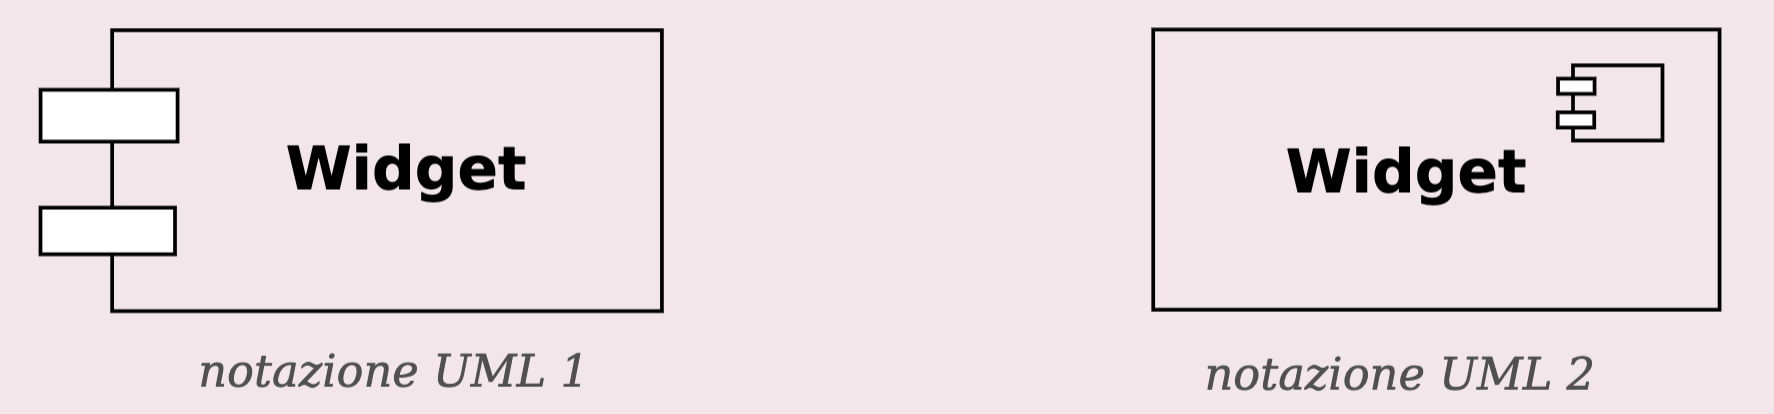
\includegraphics[width=0.75\linewidth]{assets/UML/component/component-1.png}
    \caption{Notazione componente nelle versioni UML. Un componente complesso può essere rappresentato come struttura composita.}
\end{figure}

\paragraph{Nota} I collegamenti tra componenti sono basati sulle interfacce fornite e richieste.

\begin{figure}[H]
    \centering
    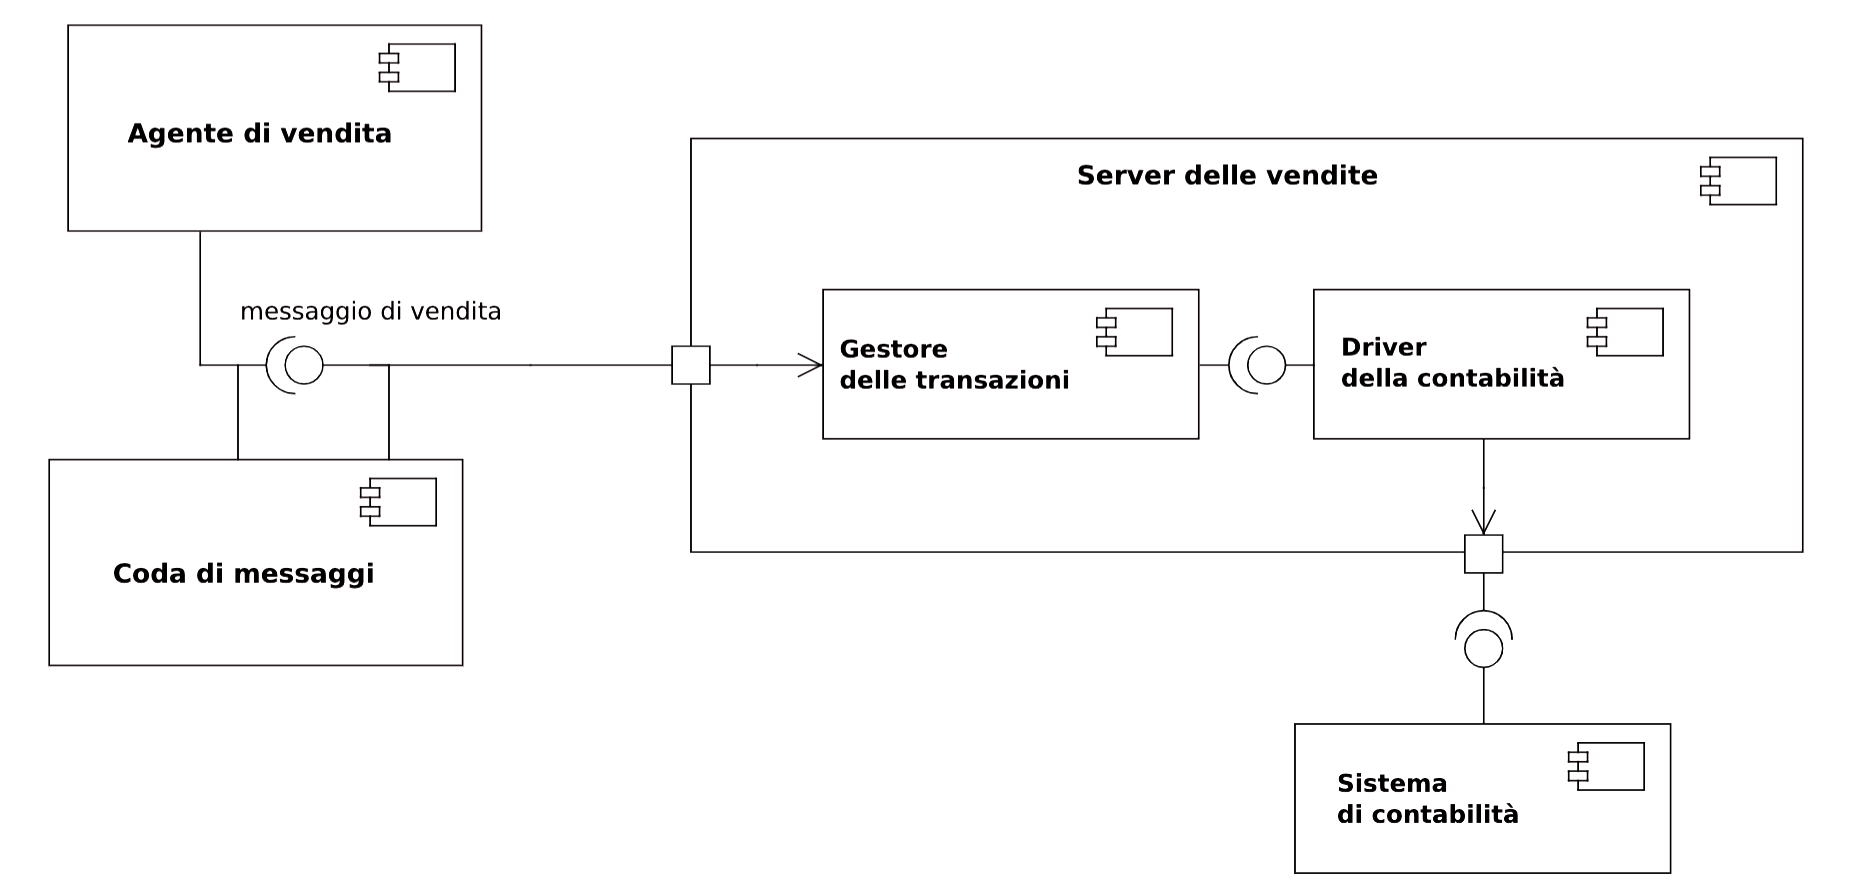
\includegraphics[width=0.75\linewidth]{assets/UML/component/component-2.png}
    \caption{Esempio di component diagram. L'agente di vendita parla: con il server se la rete è disponibile, con la coda altrimenti.}
\end{figure}

\newpage